% !Mode:: "TeX:UTF-8"
% 七年级上学期第一单元几何体的展开与折叠

\begin{defproblem}{7NJ-04-01}%
\begin{onlyproblem}%
如图是一个正方体的表面展开图,如果将它折叠成原来的正方体,那么与边LK重合的边是(    ) 
\begin{center}
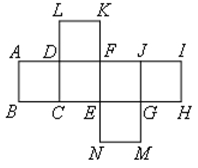
\includegraphics[width=3.5cm]{7NJ01-04-20190803-01.jpg}
\end{center}
\xx
{AB}
{FJ}
{JI}
{MN}
\end{onlyproblem}%
\begin{onlysolution}%
\begin{solution}%
选C.
\begin{center}
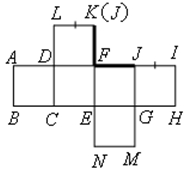
\includegraphics[width=3.5cm]{7NJ01-04-20190803-02.jpg}
\end{center}

要判断边和点的重合,需先从拐角处进行研究,再从剪开了两条棱的点处分析判断边如何重合成为棱. 一条棱与两个面相连,一条棱剪开成为两条边,一个顶点连着三条棱,一个点属于三个面. 如图,   从拐点F处开始分析,与点F相连的两条棱是连着的,剪开了一条棱,即折叠之后FK与FJ重合,点K和点J重合; 接着分析点J,与点J相连的一条棱是连着的,剪开了两条棱,得到四条边JF,JI,KL,KF,已经得出折叠后FK与FJ重合,那么剩余的KL与JI重合,即与边LK重合的边是JI. 故选C. 
\end{solution}%
\end{onlysolution}%
\end{defproblem}





\begin{defproblem}{7NJ-04-02}%
\begin{onlyproblem}%
将下图正方体的相邻两面各划分成九个相同的小正方形,并分别标上“$\circ$”、“$\times$”两符号.若下列有一图形为此正方体的展开图,则此图为(    ) 
\begin{center}
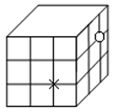
\includegraphics[width=2cm]{7NJ01-04-20190803-03.jpg}
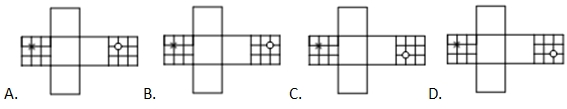
\includegraphics[width=11cm]{7NJ01-04-20190803-10}
\end{center}
\end{onlyproblem}%
\begin{onlysolution}%
\begin{solution}%%
C.
从相对面、相邻面无法判断. 再分析棱,四个展开图经过折叠,带特殊图案的两个面是相邻的.如下图,立体图中面“ABCD”和面“ABEF”有一条重合的棱AB,并且“$\times$”与棱AB的距离是1个网格,“$\circ$”与棱AB的距离是2个网格,可以排除选项B和D; 由于“$\times$”和“$\circ$”距离上下底面的高度不同,排除选项A,故选C. 

\end{solution}%
\end{onlysolution}%
\end{defproblem}



\begin{defproblem}{7NJ-04-08}%
\begin{onlyproblem}%
如图是一个正方体纸盒的表面展开图,下图能由它折叠而成的是哪一个? 
\begin{center}
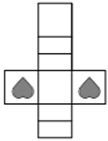
\includegraphics[width=2cm]{7NJ01-04-20190803-11}
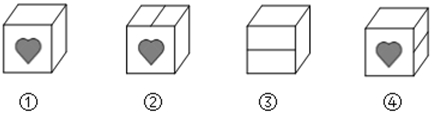
\includegraphics[width=10cm]{7NJ01-04-20190803-05.jpg}
\end{center}
思路分析 

判断正方体展开与折叠问题时,我们按照面、棱、顶点的顺序分析. 首先观察面,由展开图知相对面为“空白对空白”,“横线对横线”,“心对心”;根据“相对面不能相邻”,排除\underline{\hspace*{2cm}}和\underline{\hspace*{2cm}}. 其次研究棱的对应,“心”所在面与“横线”所在面相交于一条棱,根据“心”与这条棱的位置关系可排除\underline{\hspace*{2cm}},应选\underline{\hspace*{2cm}}. 以上横线处依次所填正确的是(    ) 

\xx
{①③④②}
{①④③②}
{①②④③}
{①③②④}
\end{onlyproblem}%
\begin{onlysolution}%
\begin{solution}%%
A.

\end{solution}%
\end{onlysolution}%
\end{defproblem}




\begin{defproblem}{7NJ-04-03}%
\begin{onlyproblem}%
如图所示的正方体的表面展开图可能是(    ) 
\begin{center}
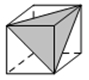
\includegraphics[width=2cm]{7NJ01-04-20190803-06.jpg}
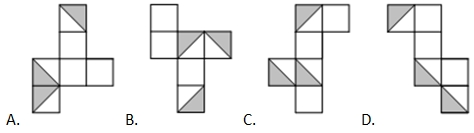
\includegraphics[width=7cm]{7NJ01-04-20190803-07}
\end{center}


\end{onlyproblem}%
\begin{onlysolution}%
\begin{solution}%%
D.
\begin{center}
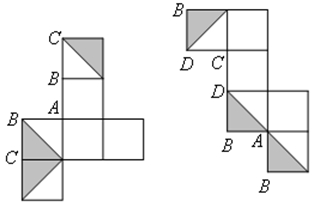
\includegraphics[width=6cm]{7NJ01-04-20190803-08}
\end{center}
先从面开始分析,带阴影的三角形的三个面是相邻面,相邻的面不可能相对,排除选项B和C. 再从棱开始分析,正方体的三个带阴影的直角三角形有公共边,并且有一个公共的顶点是直角顶点,根据一条棱与两个面相连,一条棱被剪开成为两条边,一个顶点连着三条棱,一个顶点属于三个面,分析重合的棱和顶点,选项A和D中重合的边和点如图所示,排除选项A.    故选D. 
\end{solution}%
\end{onlysolution}%
\end{defproblem}




\begin{defproblem}{7NJ-04-04}%
\begin{onlyproblem}%
将棱长为1的小正方体组成如图所示的几何体,已知该几何体共由8个小正方体组成,则该几何体的表面积是(    )平方单位. 
\begin{center}
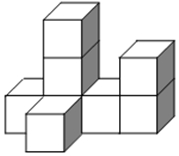
\includegraphics[width=3cm]{7NJ01-04-20190803-09}
\end{center}

\xx
{34}
{32}
{27}
{25}

\end{onlyproblem}%
\begin{onlysolution}%
\begin{solution}%%
A. 根据三视图中小正方体的个数和凹进去的部分, 几何体的表面积为$[(7+4+5) \times 2+2] \times 1^{2}=34$. 故选A. 
\end{solution}%
\end{onlysolution}%
\end{defproblem}






